\section{Distributed Processing of Spatial Algorithms}
\label{sec:spatial_dist}

\subsection{Data Structures for Spatial Data Processing}

	Spatial data objects often cover areas in multi-dimensional spaces and are not well represented by point locations For example, map objects like counties, census  tracts etc occupy regions of non-zero size  in two dimensions A common operation on spatial data is a search for all objects in an area, for example to find all counties that have land within 20 miles of a particular point. This kind of spatial search occurs frequently ii computer aided design (CAD) and geo-data applications, and therefore it is important to be able to retrieve objects efficiently according to their spatial location. 
	
	An index based on objects' spatial locations is desirable, but classical one-dimensional database indexing structures are not appropriate to multi-dimensional spatial searching structures based on exact matching of values, such as hash tables, are not useful because a range search is required Structures using one-dimensional ordering of key values, such as B-trees and ISAM indexes, do not work because the search space is multl-dimensional. 
		
	A number of structures have been proposed for handling multi-dimensional point data, such as: KD-Tree \cite{bentley1975multidimensional}, Hilbert R-Tree \cite{kamel1994hilbert} and R-Tree \cite{guttman1984r}.
	
	R-Trees were proposed by Antonin Guttman in 1984 and have found significant use in both theoretical and applied contexts, they are tree data structures used for spatial access methods, i.e, for multi-dimensional information such as geographical coordinates, rectangles, polygons. Similar to the B-Tree \cite{comer1979ubiquitous}, the R-Tree is also a balanced search tree (so all leaf nodes are at the same height).

	The key idea of the data structure is to group nearby objects and represent them with their minimum bounding rectangle (MBR) in the next higher level of the tree. Since all objects lie within this bounding rectangle, a query that does not intersect the bounding rectangle also cannot intersect any of the contained objects. At the leaf level, each rectangle describes a single object; at higher levels the aggregation of an increasing number of objects. This can also be seen as an increasingly coarse approximation of the data set.

Figure 1 illustrates the hierarchical structure of an R-Tree with a root node, internal nodes (N1...2 C N3...6) and leaves (N3...6 C a...i). The Upper Top of Figure 1 shows MBRs grouping spatial objects of a..a i in sets by their co-location. The bottom of Figure 1 illustrates the R-Tree representation. Each node stores at most M and at least m <=M/2 entries [Guttman 1984].

\begin{figure}[ht]
\centering
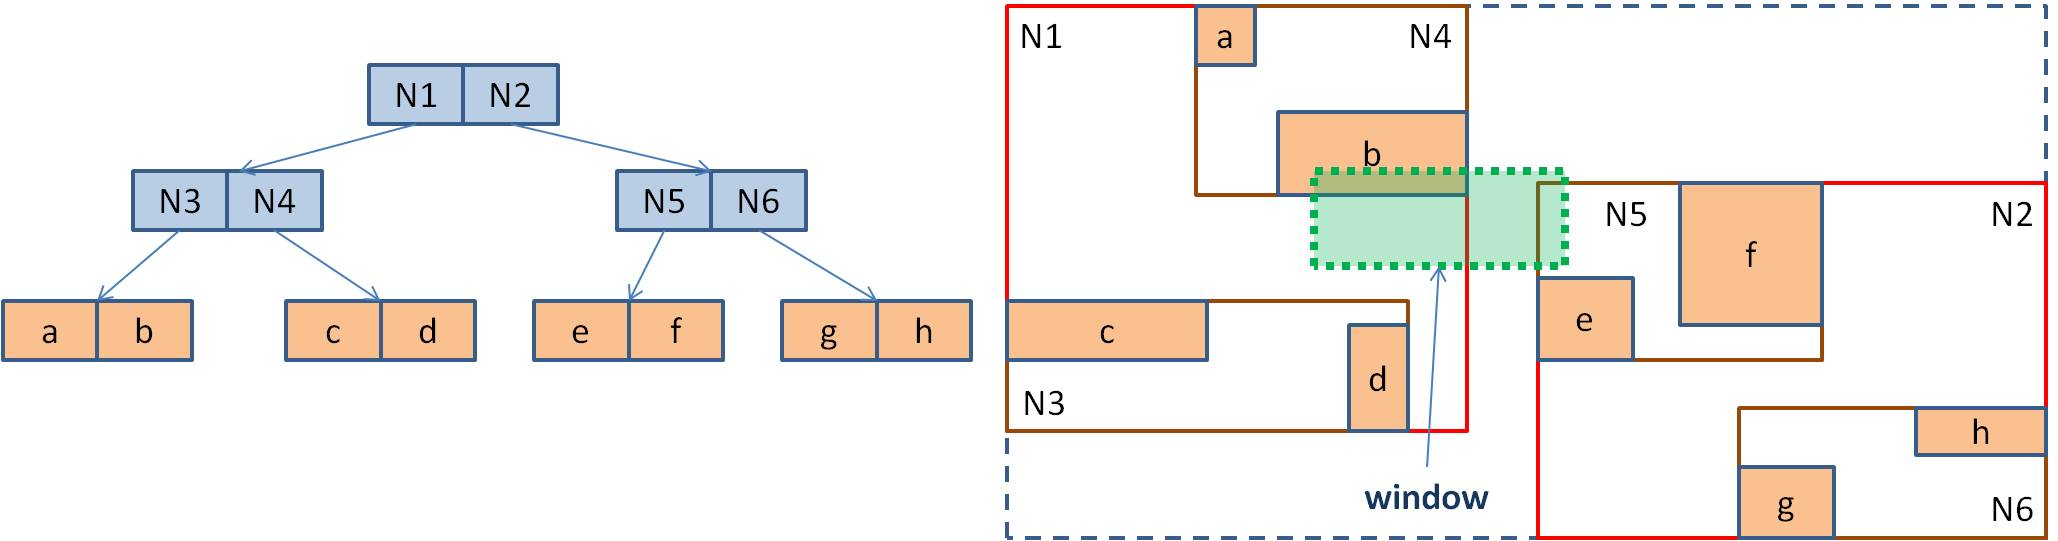
\includegraphics[width=.5\textwidth]{r-tree-structure.png}
\caption{R-Tree Structure}
\label{fig:R-Tree Structure}
\end{figure}

The input is a search rectangle (Query box). Searching is quite similar to searching in a B+ tree. The search starts from the root node of the tree. Every internal node contains a set of rectangles and pointers to the corresponding child node and every leaf node contains the rectangles of spatial objects (the pointer to some spatial object can be there). For every rectangle in a node, it has to be decided if it overlaps the search rectangle or not. If yes, the corresponding child node has to be searched also. Searching is done in a recursively until all overlapping nodes have been traversed. When a leaf node is reached, the contained bounding boxes (rectangles) are tested against the search rectangle and their objects (if there are any) are put into the result set if they lie within the search rectangle.
	
	Dead space is a space which is indexed but does not contain data. In Figure 1, N1 area is an example of dead space. Dead spaces cause the search go into false sub-trees. In figure 1, window K represents the intersection between the MBR dead space and N2, the search walks through the sub-tree of N2, although this sub-tree does not contain any data to return.
Overlapping areas are regions of intersection between polygons. The area between N3 and N4 in Figure 1 is an example of overlapping. Less overlapping reduces the amount of sub-trees accessed during r-tree traversal. The overlapping area between N3 and N4 in Figure 1, forces the traversal of the two sub-trees, degrading the performance of R-Tree \cite{beckmann1990r}.

\subsection{DistGeo: A Platform of Distributed Spatial Operations for Geoprocessing}

There are two important requirements for processing data in shared-nothing (cluster) [DeWitt and Gray 1992] architectures, First divide the data in partitions. The second requirement is distribute this partitions in the cluster nodes. For spatial datasets, we use the same idea of partitions, and the partitions distribution considers the geographic co-location among the polygons to speed up the searching algorithm.

Figure \ref{fig:partitioning} illustrates the structure of a Distributed R-Tree in a cluster. The partitioning it is performed grouping the nodes in cluster and creating the indexes according to the R-Tree structure. The lines in Figure \ref{fig:partitioning} show the need for message exchange to reach the sub-trees during the algorithm processing.

\begin{figure}[ht]
\centering
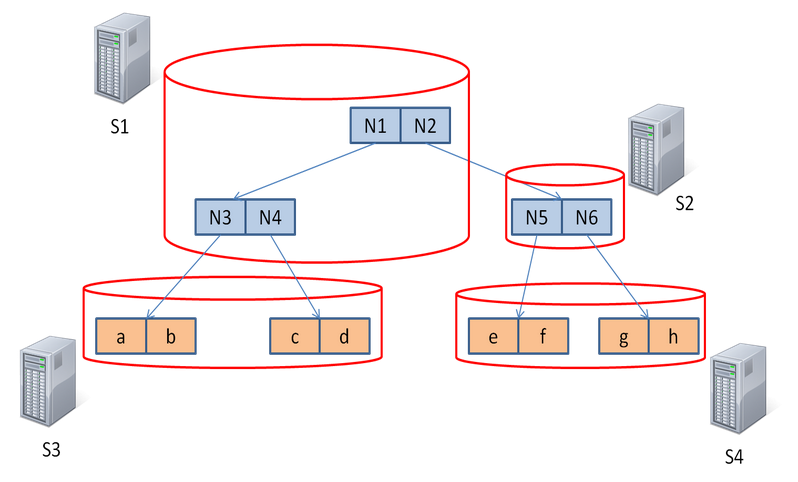
\includegraphics[width=.5\textwidth]{r-tree-partiotioning.png}
\caption{R-Tree Partitioning in a shared-nothing architecture}
\label{fig:partitioning}
\end{figure}

Insertions and searching in a distributed R-Tree are similar to the non-distributed version, except for:
i) The need of message exchange to access the distributed partitions
ii) Concurrency control and consistency due to the parallel processing in the cluster.
	The data distribution among the distributed partitions in the cluster is both the main factor to the parallel processing and also the main challenge when building the distributed index.
	Quality of index is another factor, which influences the communication. An index with high quality reduces the searching space and the sub-tress access leading to less number of message exchange.
	This section describes the main architecture decisions and some implementation details that molds the challenges when constructing a solution for distributed Geo-processing.
	The distributed index has been built according to the taxonomy defined in [An et al. 1999], as follows:
	i) Allocation Unit: block - A partition is created for every R-Tree node;
	ii) Allocation Frequency: overflow - In the insert process, new partitions are created when a node in the tree needs to split;
	iii) Distribution Policy: balanced - To keep the tree balanced the partitions are distributed among the cluster nodes.
	DistGeo is based on the shared-nothing architecture, which the nodes do not share CPU, hard disk and memory and the communication relies on message exchange. Figure 3 depicts DistGeo plataform based on peer-to-peer model, with the data manage by the cluster presented as a ring topology. It is divided in ranges of keys, which are managed for each node of the cluster. To a node join the ring it must first receive a range
	The range of keys are known by each node in the cluster. For instance, in a ring representation, whose key set start with 0 till 100, if we have 4 nodes in the cluster, the division would be done as shown below:
\begin{enumerate}
 \item node 1: 0-25
  \item node 2: 25-50
  \item node 3: 50-75
  \item node 4: 75-100
\end{enumerate}

If we want to search for one object with key 34, we certainly should look on the node 2.

\begin{figure}[ht]
\centering
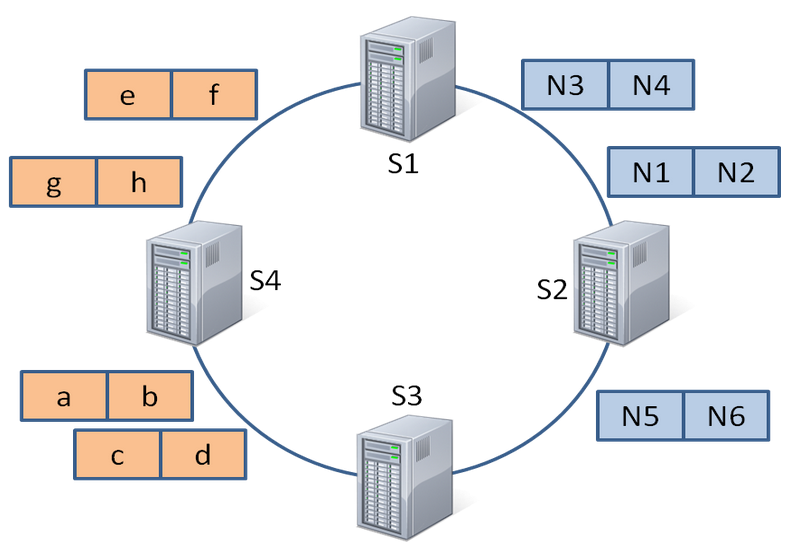
\includegraphics[width=.5\textwidth]{figure3.png}
\caption{Figure 3}
\label{fig: Figure 3}
\end{figure}

	Reliability and fault-tolerance are implemented storing the R-Tree nodes in multiple nodes in the cluster. Each node N receives a key, which is used to store the node in a server S responsible for ring range, replicating the node N to the next two servers in S (clockwise).
	
	Data replication is equally important. If a message is sent to a bode N, in the moment of R-Tree traversal an active server is elected, and replicates the data in this node to further requisition processing.
	
	The Gossip protocol, which every cluster node exchanges information among themselves is used by DistGeo for service discovery and knowing the status of the cluster's nodes. Gossip protocol. Every second a message is exchanged among three nodes in the cluster, consequently every cluster's node have knowledge of each other.
	
	Read/Write operations may be performed in any node of the cluster. When a request is made to a cluster's node, it becomes the coordinator of the operation requested by the client. The coordinator works as a proxy between the client and the cluster's nodes. In a distributed R-Tree, the requests are always sent to cluster's node, which stores the root node of the R-tree.